\documentclass[12pt]{article}
\usepackage{titlesec}
\usepackage{bm}
\usepackage{amsmath}
\usepackage{amsfonts}
\usepackage{amssymb}
\usepackage{graphicx}
\usepackage{colortbl}
\usepackage{xr}
\usepackage{hyperref}
\usepackage{longtable}
\usepackage{xfrac}
\usepackage{tabularx}
\usepackage{float}
\usepackage{siunitx}
\usepackage{booktabs}
\usepackage{array}
\usepackage{fullpage}
\usepackage[round]{natbib}
\usepackage{multirow}
\usepackage{booktabs}
\usepackage{graphicx}
\usepackage{array}

\newcolumntype{C}[1]{>{\centering\let\newline\\\arraybackslash\hspace{0pt}}m{#1}}
\graphicspath{ {images/} }


\hypersetup{
   bookmarks=true,         % show bookmarks bar?
     colorlinks=true,       % false: boxed links; true: colored links
   linkcolor=black,          % color of internal links (change box color with linkbordercolor)
   citecolor=green,        % color of links to bibliography
   filecolor=magenta,      % color of file links
   urlcolor=cyan           % color of external links
}
\newcommand{\wss}[1]{\authornote{magenta}{SS}{#1}}
\newcommand{\hed}[1]{\authornote{blue}{HM}{#1}} %Hediyeh
\newcommand{\tz}[1]{\authornote{blue}{TZ}{#1}} %Tahereh
\newcommand{\pl}[1]{\authornote{blue}{PL}{#1}} %Peng

\newcommand{\colZwidth}{1.0\textwidth}
\newcommand{\blt}{- } %used for bullets in a list
\newcommand{\colAwidth}{0.13\textwidth}
\newcommand{\colBwidth}{0.82\textwidth}
\newcommand{\colCwidth}{0.1\textwidth}
\newcommand{\colDwidth}{0.05\textwidth}
\newcommand{\colEwidth}{0.8\textwidth}
\newcommand{\colFwidth}{0.17\textwidth}
\newcommand{\colGwidth}{0.5\textwidth}
\newcommand{\colHwidth}{0.28\textwidth}
\newcounter{defnum} %Definition Number
\newcommand{\dthedefnum}{GD\thedefnum}
\newcommand{\dref}[1]{GD\ref{#1}}
\newcounter{datadefnum} %Datadefinition Number
\newcommand{\ddthedatadefnum}{DD\thedatadefnum}
\newcommand{\ddref}[1]{DD\ref{#1}}
\newcounter{instnum} %Instance Number
\newcommand{\itheinstnum}{IM\theinstnum}
\newcommand{\iref}[1]{IM\ref{#1}}
\newcounter{reqnum} %Requirement Number
\newcommand{\rthereqnum}{P\thereqnum}
\newcommand{\rref}[1]{R\ref{#1}}
\newcounter{lcnum} %Likely change number
\newcommand{\lthelcnum}{LC\thelcnum}
\newcommand{\lcref}[1]{LC\ref{#1}}

\newcommand{\tclad}{T_\text{CL}}
\newcommand{\degree}{\ensuremath{^\circ}}
\newcommand{\progname}{SWHS}

\usepackage{fullpage}

\begin{document}

\begin{titlepage}
\font\myfont=cmr12 at 38pt
\title{\myfont\vspace{60mm}Zop Test Plan}
\author{Ratna Emani, Cole Blanchard, Akshay Mantha}
\date{\today}
\maketitle

\end{titlepage}

\newpage
\textbf{Revision History}\\
\begin{center}
\begin{tabular}{|C{3cm}|C{3cm}|C{3cm}|C{3cm}|}
\hline
\textbf{Developer} & \textbf{Date} & \textbf{Change} & \textbf{Revision Number}\\
\hline \hline
Cole Blanchard & November 27 2015 & Robustness Testing, \newline Performance Testing, \newline Traceability Matrix & 4\\
\hline
Ratna Emani & November 27 2015 & Reliability,\newline Maintainability, \newline Correctness, Ease of Use,\newline 3.4 Raw Game-play Test & 3\\
\hline
Akshay Mantha & November 27 2015 & System Tests & 2\\
\hline
Ratna Emani & November 27 2015 & Traceability to modules, \newline Formatting, \newline Approach, \newline Usability Testing & 1\\
\hline
\end{tabular}
\end{center}

\newpage
\tableofcontents
\newpage


\section{Introduction}


\subsection{Approach}

	Performance testing gives the programmers a sense of how efficiently their implemented methods and functions are being used throughout the program.  This efficiency can be measured in a variety of ways which includes the average time it take to execute each function or looking at the average number of times the function has been called throughout the program.  This can give the programmers an idea of where the program can be improved such as reducing the number of comparisons a function makes, or reducing the out of memory a function is using.\\

Usability testing allows other users to play the game and experience the functional game before it reaches its final stage. This is very important to the development process so the development team can see the user expectations and reactions first hand before they unveil the final product. Allowing for some important changes/additions to the implementation. During the development phase companies conduct similar testing called, Alpha testing. Alpha testing allows the development team to pick and fix any bugs that appear in the game. The selected participants usually involve employees and sometimes family/friends, to emulate 80\% of the customers.\\
 
Unit testing is an important tool for testing out basic methods and functions of modules. It is a simple, yet powerful tool that provides the user with comprehensive coverage and quality assurance of the fundamental code of a given program. We decided that Logic.py is a module that needs to be tested the most since it has methods, which are responsible for a working game. Thus, we covered it in depth. Also, we made sure to do a test case that takes care of constructing a board (of proper size; 6 by 6) with tiles. Unit testing has helped our team validate our project.


\section{Traceability to modules}
 
\begin{table}[h!]
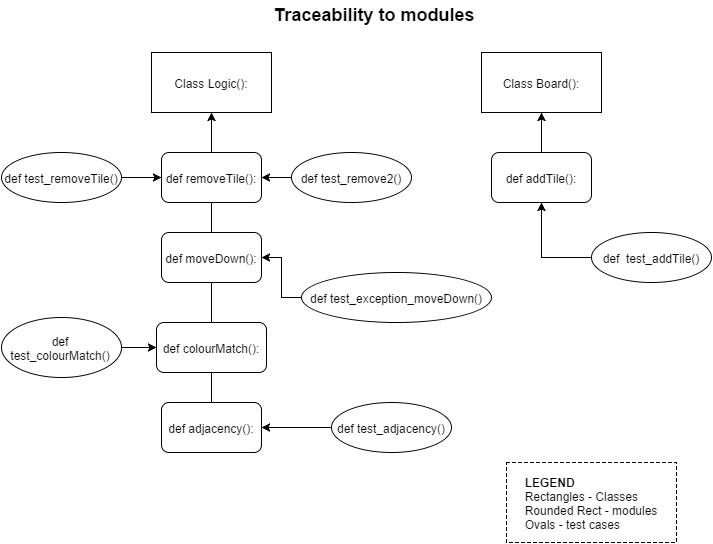
\includegraphics[width = 17cm]{traceModules}
\caption{Traceability to Modules}
\end{table}


\newpage


\section{System Tests}
%3.1 Number of Tiles Removed and Score Are the Same
\subsection{Tile(s) Removed and Value is set to 0}

\subsubsection{Test type}
Automated, unit test

\subsubsection{Initial state}
The board is initialized, size of 6 by 6; 36 blocks in place.

\subsubsection{Input}
Tile(s) removed (after matching).

\subsubsection{Expected Output}
The value of tile(s) removed is 0.

\subsubsection{Test Result}
PASS.

\newpage

%3.2 Number of Tiles Removed and Score are Not the Same
\subsection{Tile(s) Removed and Value is not 0}
\subsubsection{Test type}
Automated, unit test

\subsubsection{Initial state}
The board is initialized, size of 6 by 6; 36 blocks in place.

\subsubsection{Input}
Tile(s) removed (after matching).

\subsubsection{Expected Output}
The value of tile(s) removed is not 0.

\subsubsection{Test Result}
PASS.

\newpage

%3.3 Colour Match of Tiles
\subsection{Colour Match of Tiles}
\subsubsection{Test type}
Automated, unit test
\subsubsection{Initial state}
The board is initialized, size of 6 by 6; 36 tiles in place.
\subsubsection{Input}
Coordinates of tiles are given to the function.
\subsubsection{Expected Output}
A boolean value; true when the selected blocks' colour is the same.

\subsubsection{Test Result}
PASS (if colour of tiles is same)/ FAIL (if colour of tiles is not the same).
Note: The Test Result can be, both, PASS or FAIL because of the "random" nature of colour.


\newpage

\subsection{Board Update Test}
\subsubsection{Test type}
Automated, Structural test

\subsubsection{Initial state}
State after removing tiles from the board (some spaces are empty).

\subsubsection{Input}
6x6 array (empty spaces flagged).

\subsubsection{Expected Output}
6x6 array (no empty spaces remaining, tiles above move down to fill empty spaces.

\subsubsection{Test Result}
PASS.

\newpage

%3.5 Board Update Test
\subsection{Tile Adjacency Check}
\subsubsection{Test type}
Automated, unit test

\subsubsection{Initial state}
Board is initialized, 6x6 array.

\subsubsection{Input}
Coordinates of blocks are given

\subsubsection{Expected Output}
Boolean value is given; True when blocks are directly next to each other, False otherwise.

\subsubsection{Test Result}
PASS.

\newpage

%3.6 Tile Adjacency Check
\subsection{Type Exception Check (While Moving Tiles Down)}
\subsubsection{Test type}
Automated, unit test
\subsubsection{Initial state}
Board is initialized, 6x6 array.
\subsubsection{Input}
Column number, instance of board, and an integer representing the number of empty spaces (in a column). 
\subsubsection{Expected Output}
Assertion should throw a 'TypeError' if either the column number is not an integer, some other object/class is instantiated instead of board, and there is no integer to represent the number of empty spaces (in a column).
\subsubsection{Test Result}
PASS.

\section{Traceability Matrix}
\begin{table}[H]
\centering
\begin{tabular}{p{0.4\textwidth} p{0.6\textwidth}}
\toprule
\textbf{Test} & \textbf{Requirement}\\
\midrule
test removeTile & Select game piece\\
test checkColumn & Must correctly display new board when tiles are deleted\\
test moveDown & Must correctly display new board when tiles are deleted\\
test addTile & Must correctly display new board when tiles are deleted\\
test colourMatch & Delete selected pieces of same colour\\
test adjacent & Delete selected pieces that are adjacent\\
performance tests & Must run in reasonable time (no delay/lag)\\
usability tests & 80\% of users should easily understand how to play\\

\bottomrule
\end{tabular}
\caption{Traceability Matrix}
\end{table}


\section{Performance Testing}
This section will be highlighting the performance of the function in the Logic class.  Each function was tested throughout 10 playthroughs giving the average number of times the function was called within the average 60 second game of Zop.
\begin{table}[h!]
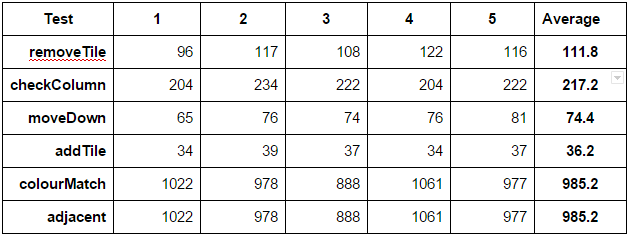
\includegraphics[width = 17cm]{perfTable}
\caption{Function Calling Count}
\end{table}
					

\subsection{Performance test: removeTile}
removeTile is called everytime a player selects a piece.  So, this number should reflect the score the player ends up with at the end of each game.  However, when the player selects only one piece, this does not add to the score.  The number of times removeTile is called will always be equal or slightly higher than the score the player achieve during the game. \\
\textbf{Results: } Called an average of 111.8 times per game of Zop

	
\subsection{Performance test: checkColumn}
checkColumn is called everytime the player finishes a turn.  It checks each column, so it is called a total of 6 times each time addTile is called.  Therefore the number of times checkColumn is called is always 6 times the number of valid (selecting more than one piece) turns the player makes.\\
\textbf{Results: } Called an average of 217.2 times per game of Zop

\subsection{Performance test: moveDown}
moveDown is called everytime the player finishes a turn. It is called whenever addTile is called.  However, the number of times the function is called varies in each game.  This is due to the randomness of Zop, meaning that selecting a certain number of tiles, or selecting the tiles in a certain direction can give different numbers.  A rough estimate of how many times this function is called is roughly twice the number of valid turns the player makes.\\
\textbf{Results: } Called an average of 74.4 times per game of Zop

\subsection{Performance test: addTile}
addTile is called everytime the player finishes a turn.  It uses functions checkColumn and moveDown.  This function is called whenever the player makes a valid turn.  The number of times this function is called is a 1:1 ratio when compared to the number of valid turns the player makes.\\
\textbf{Results: } Called an average of 36.2 times per game of Zop

\subsection{Performance test: colourMatch and adjacent}
colourMatch and adjacent are called whenever a selected tile is compared to any other new tile the player has hovered over with their mouse.  This number depends on how sporadic the player is playing.  If the player hovers over many tiles that give False comparisons the number of times these functions can potentially be called may reach very high numbers.  However a player making calculated moves can lower this number drastically.  The number of times these functions are called depends on user tendencies.\\
\textbf{Results: } Called an average of 985.2 times each per game of Zop

\section{Usability Testing}
For the usability test cases we decided to ask a team of four individuals. After playing Zop each of them gave their personal opinions and recommendations to make the game more interactive and overall likeable. The feedback responses were are great way of testing the GUI*. User feedback is very vital, as more of it is implemented the more likeable the application becomes. However with a deadline nearby, it is important for the development team to prioritize the feedback appropriately.\\\\
\textbf{User \# 1:}
Marcus\\
\textbf{Bio:}
Enjoys reading and playing a lot of mobile games.\\
\textbf{Feedback:}
\begin{itemize}
 \item User input is slow and unintuitive, the user wastes a lot of time in selecting the tiles. (High Priority)
 \item Background flashes Red when game has 10 secs left, to increase interactivity and also helps keep the player engaged. (Medium Priority)
\item Make the size of the grid larger by another column and row, and change the rule to connect a minimum of 3 tiles. (Medium Priority)
\item Add more interactive images/sprites and sounds to make the overall application more appealing. (Medium Priority)
 \item Bonus points are awarded to the player if they connect tiles in the shape of a square. (Low Priority)
\end{itemize}
\textbf{User \# 2:}
Harry\\
\textbf{Bio:}
Likes challenges and enjoys games on all platforms.\\
\textbf{Feedback:}
\begin{itemize}
 \item User likes the change from the unintuitive single tile clicking. (Fixed)
\item Noticeable lag when mouse click is too fast. (High Priority)
\item Display Personal Score at the end screen. (High Priority)
\item Suggested to add sound files to the game to increase interactivity. (Medium Priority)
\item Add quick instructions on the start Menu. (Medium Priority)
\end{itemize}
\textbf{User \# 3:}
Sid\\
\textbf{Bio:}
Very active, enjoys a lot of sports and playing Wii.\\
\textbf{Feedback:}
\begin{itemize}
 \item Although dragging the mouse is better it can sometimes lag when the input is entered too fast. (High Priority)
\item Show the top 5 player scores on the end screen. (High Priority)
\item Display player score and the overall rank at the end screen. (High Priority)
\item Add a main menu and a restart button to the end screen. (High Priority)
\item Suggested to make the size of the tiles smaller. (Medium Priority)
\end{itemize}
\textbf{User \# 4:}
David\\
\textbf{Bio:}
Very busy with office work, usually spends time gaming on weekends or mostly on his phone.\\
\textbf{Feedback:}
\begin{itemize}
 \item Not smooth however playable when slow/steady when selecting and dragging over tiles (Potential Fix)
\item Show the top 5 player scores on the end screen .(High Priority)
\item There can be a bonus round added to make the game more versatile. (Low Priority)
\item The player gets awarded extra seconds of time as they score more tiles. (Low Priority)
\item The greater combination of tiles increase the total time awarded.  (low Priority)
\end{itemize}

The usability testing will have a great impact on our final product during the final demonstration. Every person who tried the game had some feedback that can drastically improve the game and some suggestions that would make the overall game more entertaining. Therefore the feedback has been separated into three tiers: High, Medium and Low Priority. 

High priority, means that the feedback is easy to implement, and/or is critical to the core gameplay. It may also include any requirements that have not been covered. For example, our original model of the game received a single click per tile to register it as a point. However, users felt that this slowed the gameplay down too much. Therefore the input was changed from single tile clicking to dragging over tiles, which yielded a positive response from the users. 

Medium priority suggestion are not completely necessary for the game completion. However, medium priority feedback is usually small changes made to the design or the rules of the game, to make it more interesting. One of the participating users, Marcus, had a lot of ideas to make the game more engaging and fun. He believed that the game is too bland to play and be engaging due to its linear rules. He suggested miniscule changes such as expanding the board by a column and a row, and change the requirement from minimum number of selected tiles from 2 tiles to 3 tiles. He also suggested another requirement; rewarding players bonus points for making squares when selecting tiles.

Finally low priority feedback is usually implemented when all necessary changes have been made and the game is fully functional. Many users agreed that adding sounds to the overall gameplay can make it more engaging and entertaining. Changes requested with low priority are usually implemented much later, or at least after the first rollout. It can have a new set of requirements that changes the rules, to add different versions to the game. David suggested adding another game style, where users should be awarded bonus time (in seconds) besides their score. This will give the user incentive to collect larger combinations of tiles for more points and time. 

\section{Robustness Testing}
Robustness testing was NOT needed to test Zop.  This is due to the fact there are no boundary conditions that the program can overreach.  The game is played in a contained window with sets limits of where and what the user inputs into the game.  There is also a set timer of 60 seconds which cannot countdown past 0 and score which cannot be too high of a number due to the 60 seconds limit.  Robustness is a good option for programs such as calculators where integer addition can create overflow but concerning Zop, robustness testing is not necessary.
\end{document}

